\PassOptionsToPackage{unicode=true}{hyperref} % options for packages loaded elsewhere
\PassOptionsToPackage{hyphens}{url}
%
\documentclass[
]{article}
\usepackage{lmodern}
\usepackage{amssymb,amsmath}
\usepackage{ifxetex,ifluatex}
\ifnum 0\ifxetex 1\fi\ifluatex 1\fi=0 % if pdftex
  \usepackage[T1]{fontenc}
  \usepackage[utf8]{inputenc}
  \usepackage{textcomp} % provides euro and other symbols
\else % if luatex or xelatex
  \usepackage{unicode-math}
  \defaultfontfeatures{Scale=MatchLowercase}
  \defaultfontfeatures[\rmfamily]{Ligatures=TeX,Scale=1}
\fi
% use upquote if available, for straight quotes in verbatim environments
\IfFileExists{upquote.sty}{\usepackage{upquote}}{}
\IfFileExists{microtype.sty}{% use microtype if available
  \usepackage[]{microtype}
  \UseMicrotypeSet[protrusion]{basicmath} % disable protrusion for tt fonts
}{}
\makeatletter
\@ifundefined{KOMAClassName}{% if non-KOMA class
  \IfFileExists{parskip.sty}{%
    \usepackage{parskip}
  }{% else
    \setlength{\parindent}{0pt}
    \setlength{\parskip}{6pt plus 2pt minus 1pt}}
}{% if KOMA class
  \KOMAoptions{parskip=half}}
\makeatother
\usepackage{xcolor}
\IfFileExists{xurl.sty}{\usepackage{xurl}}{} % add URL line breaks if available
\IfFileExists{bookmark.sty}{\usepackage{bookmark}}{\usepackage{hyperref}}
\hypersetup{
  pdftitle={Measuring distances from the frontier},
  pdfauthor={Irena Papst},
  pdfborder={0 0 0},
  breaklinks=true}
\urlstyle{same}  % don't use monospace font for urls
\usepackage[margin=1in]{geometry}
\usepackage{graphicx,grffile}
\makeatletter
\def\maxwidth{\ifdim\Gin@nat@width>\linewidth\linewidth\else\Gin@nat@width\fi}
\def\maxheight{\ifdim\Gin@nat@height>\textheight\textheight\else\Gin@nat@height\fi}
\makeatother
% Scale images if necessary, so that they will not overflow the page
% margins by default, and it is still possible to overwrite the defaults
% using explicit options in \includegraphics[width, height, ...]{}
\setkeys{Gin}{width=\maxwidth,height=\maxheight,keepaspectratio}
\setlength{\emergencystretch}{3em}  % prevent overfull lines
\providecommand{\tightlist}{%
  \setlength{\itemsep}{0pt}\setlength{\parskip}{0pt}}
\setcounter{secnumdepth}{-2}
% Redefines (sub)paragraphs to behave more like sections
\ifx\paragraph\undefined\else
  \let\oldparagraph\paragraph
  \renewcommand{\paragraph}[1]{\oldparagraph{#1}\mbox{}}
\fi
\ifx\subparagraph\undefined\else
  \let\oldsubparagraph\subparagraph
  \renewcommand{\subparagraph}[1]{\oldsubparagraph{#1}\mbox{}}
\fi

% set default figure placement to htbp
\makeatletter
\def\fps@figure{htbp}
\makeatother

\usepackage[fontsize=13pt]{scrextend}

\title{Measuring distances from the frontier}
\author{Irena Papst}
\date{}

\begin{document}
\maketitle

In order to perform certain statistical analyses associated with
regression discontinuity design (RDD), one must have an appropriate
measure of distance from the frontier of the assignment region. For
simplicity, let's consider the case of two independent variables, but
the metric we derive generalizes to \(n\) independent variables.

Let \(F\) denote the frontier, composed of two thresholds \(x = c_1\)
and \(y = c_2\). Without loss of generality, assume the assignment rule
is \(x \geq c_1\) and
\(y \geq c_2\)\footnote{The subsequent analysis will still work, even if one or both inequalities are flipped and/or strict.},
hence the assignment region, \(A\) is where \textbf{both} of these rules
are satisfied. Then the frontier can be written in set notation as
\(F = \{ x = c_1 , y \geq c_2 \} \cup \{ y = c_2, x \geq c_1\}\). All of
this fancy notation simply describes the following sketch:

\begin{center}
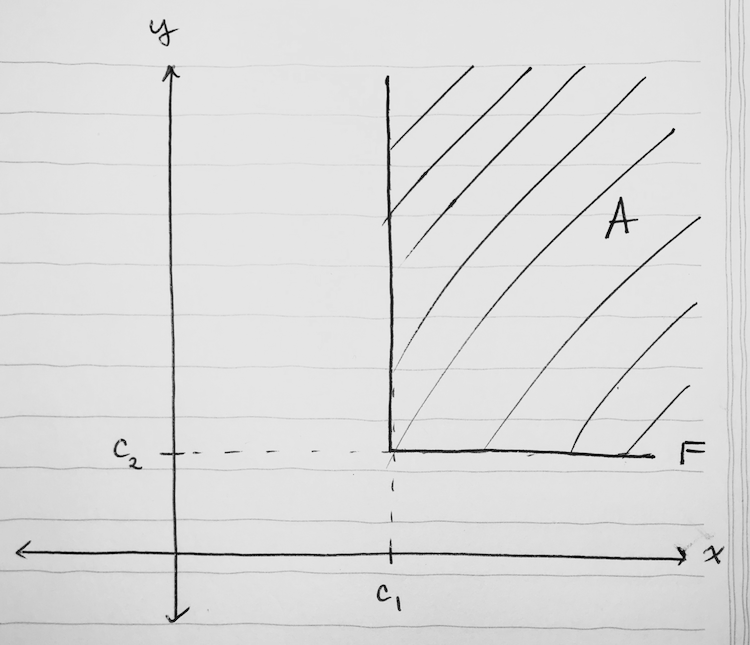
\includegraphics[width=0.6\textwidth]{figs/f1.png}
\end{center}

The question we want to answer is: what does it mean for a subject to be
\(\varepsilon > 0\) away from the frontier?

In the case where \emph{either} \(x \geq c_1\) or \(y \geq c_2\), the
solution is relatively straightforward. The subject satisfies one of the
assignment rules already, and so they only must increase (decrease) the
other independent variable by \(\varepsilon\) to reach the frontier. For
example, if \(x \geq c_1\) for a subject, then they should be considered
\(\varepsilon\) away from the frontier if their \(y\) variable is either
\(\varepsilon\) more or \(\varepsilon\) less than the threshold
\(y=c_2\). Again, a diagram clarifies this description:

\begin{center}
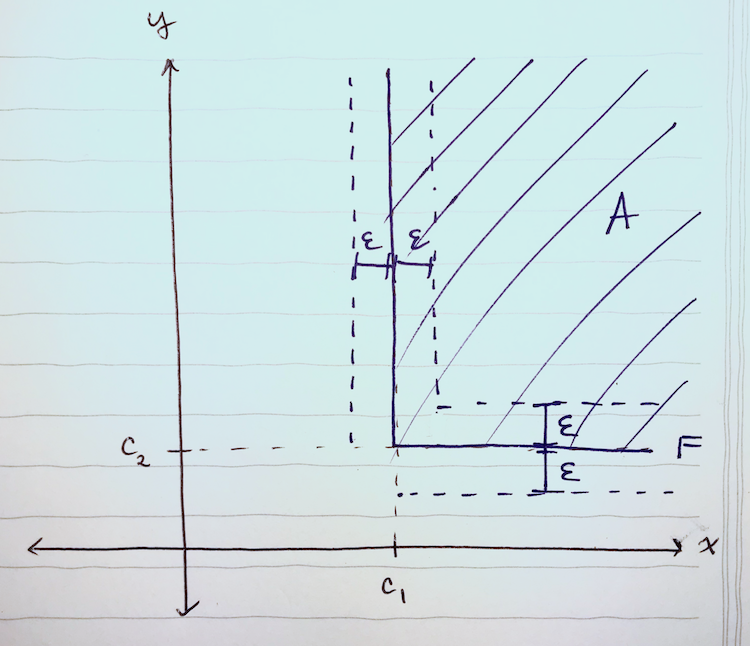
\includegraphics[width=0.6\textwidth]{figs/f2.png}
\end{center}

All the points on the blue dashed line are \(\varepsilon\) away from the
frontier F.

But what happens at the corner of the frontier; specifically on the
outside of the assignment region?

\begin{center}
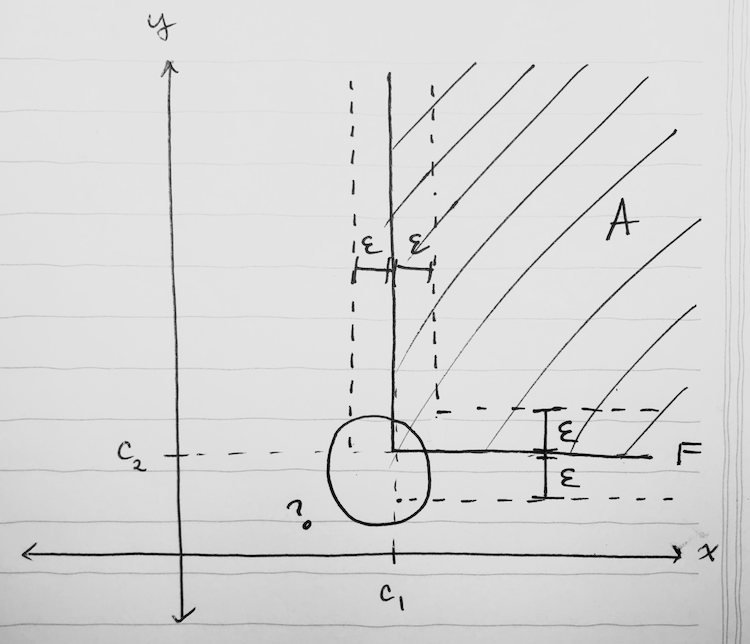
\includegraphics[width=0.6\textwidth]{figs/f3.png}
\end{center}

Here it helps if we really focus about the application. First off,
recall that \(x\) and \(y\) are independent of each other; a change in
one of these variables does not provoke a change in the other. For a
subject, that means that they can only move in horizontal and vertical
motions in this space of attributes. What we really mean when we say a
subject is \(\varepsilon\) away from the frontier, is that adding their
horizontal and vertical distance from the frontier gives
\(\varepsilon\).

We also implicitly took the \emph{minimum} distance to the frontier in
teh above cases; although we could calculate the distance between a
point and \emph{any} point on the frontier, we took the \emph{closest}
frontier point.

Using these two ideas, we can now derive the points that are
\(\varepsilon\) from the frontier in the case where \emph{both}
\(x<c_1\) and \(y<c_2\) (we are below the assignment threshold in
\emph{both} variables). First off, note that the closest frontier point
to points that satisfy these conditions is the corner \((c_1, c_2)\).
The points that are \(\varepsilon\) away from the frontier corner, using
our reasoning that subjects can only move horizontally and vertically,
would be those whose difference in \(x\)-coordinate,
\(\Delta x = |x-c_1|\), and difference in \(y\)-coordinate,
\(\Delta y = |y-c_2|\) sums to \(\varepsilon\). Such points form a
triangular buffer around the frontier corner:

\begin{center}
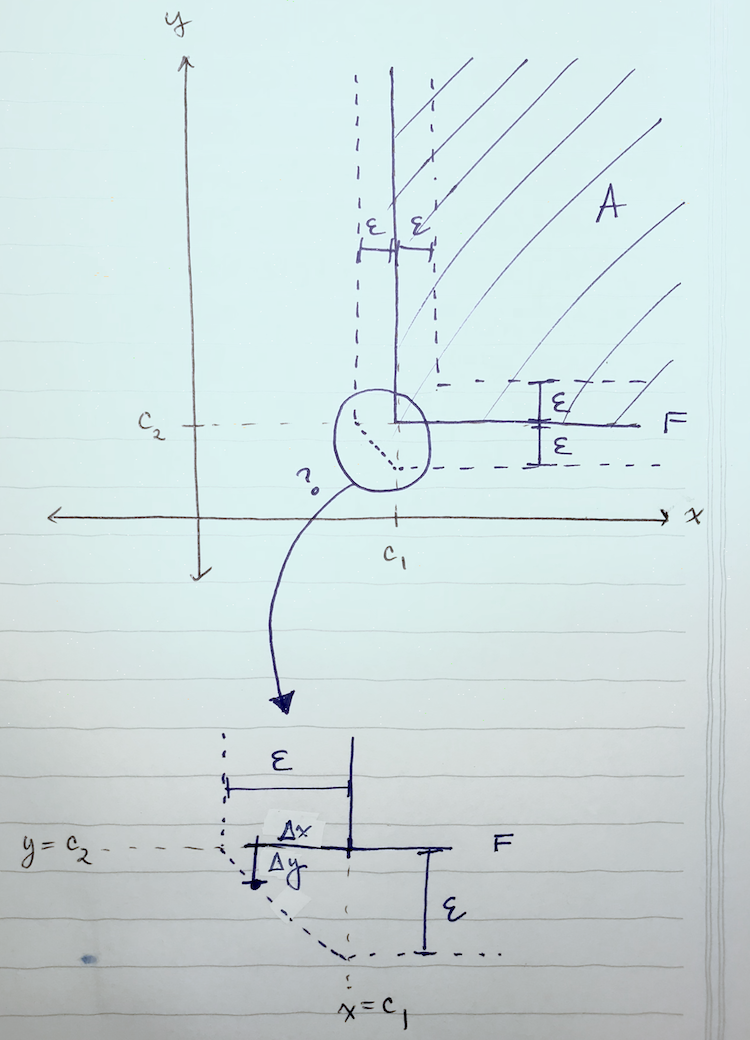
\includegraphics[width=0.6\textwidth]{figs/f4.png}
\end{center}

Formally, this is the \(l_1\)-metric to the frontier, where the distance
between a point \(p = (p_x,p_y)\) and a set, \(A\), is abstractly
defined
as\footnote{Really, this quantitiy should be phrased in terms of the \href{https://en.wikipedia.org/wiki/Infimum_and_supremum}{infimum} instead of the minimum, but I'm omitting these mathematical details here.}
\begin{align}
l_1(p,A) &= \min_{a=(a_x,a_y) \in A} \{ l_1(p,a)\} \\
&= \min_{a=(a_x,a_y) \in A} \{|p_x-a_x|+|p_y-a_y|\}.
\end{align}

For a point \(p = (p_1, p_2, ..., p_n) \in \mathbb{R}^n\) and set \(A\)
in the same space, this metric generalizes to \begin{align}
l_1(p,A) = \min_{a = (a_1, a_2, ..., a_n) \in A} \left \{ \sum_{i = 1}^n |p_i - a_i| \right \}.
\end{align}

\end{document}
